\clearpage
\setcounter{section}{5}
\section{Sequential compactness}

\topic{Sequential compactness}
\begin{note}{Definition and first consequences}
$K\subseteq E$ is sequentially compact if \emph{every} sequence in $K$ has a subsequence converging to a point of $K$. The subsequence may depend on the starting sequence. The limit-in-$K$ condition is essential.

Sequential compactness is intrinsic: inherited distances are the same, and the required limits belong to $K$, so passing to a larger ambient space does not change it. It implies closedness, boundedness and completeness.

For closedness: if $x_n\in K$ converges to $x$ in $E$, a compactness subsequence converges to $p\in K$, and uniqueness gives $x=p$. For boundedness: if unbounded, choose points with distances from a fixed point increasing to infinity; no subsequence can converge. For completeness: a Cauchy sequence has a convergent subsequence, and the Cauchy-subsequence lemma makes the whole sequence converge.
\end{note}
\begin{note}{Closed subsets, unions and intersections}
A closed subset $F$ of a sequentially compact $K$ is sequentially compact: take a subsequence converging in $K$; closedness puts the limit in $F$. Conversely every sequentially compact subset is closed. Hence within a sequentially compact ambient space, ``closed'' and ``sequentially compact'' are equivalent for subsets.

Finite sets are sequentially compact by the infinite pigeonhole principle. Finite unions of sequentially compact sets are sequentially compact: infinitely many terms lie in one constituent. Intersections of two sequentially compact sets are sequentially compact because one is closed and the intersection is a closed subset of the other. For an arbitrary nonempty family of such sets, the same closed-subset argument works using one member to bound the intersection.
\end{note}
\begin{exam}{2022 Q4(a): compact subsets of a compact space}
Let $K$ be sequentially compact and $A\subseteq K$. Prove $A$ is sequentially compact iff $A$ is closed in $K$.
\end{exam}
\begin{answer}
Suppose $A$ is sequentially compact. If $a_n\in A$ and $a_n\to x$ in $K$, there is a subsequence $a_{n_j}\to a\in A$. Since the original sequence tends to $x$, that subsequence also tends to $x$. Uniqueness gives $x=a\in A$, proving $A$ closed in $K$.

Conversely suppose $A$ closed in $K$. Any sequence in $A$ is also a sequence in $K$, so has a subsequence converging to some $x\in K$. Since every term of the subsequence lies in $A$ and $A$ is closed in $K$, $x\in A$. Thus $A$ is sequentially compact.
\end{answer}
\begin{exam}{Additional practice: complete and bounded is insufficient}
Give a complete bounded metric space which is not sequentially compact.
\end{exam}
\begin{answer}
Take $E=\N$ with the discrete metric. Its diameter is $1$, so it is bounded. Every Cauchy sequence is eventually constant, so it is complete. But the sequence $x_n=n$ has distinct terms, as does every subsequence. A convergent sequence in a discrete space must be eventually constant, so this sequence has no convergent subsequence. Hence $E$ is not sequentially compact.
\end{answer}
\begin{tip}
Completeness controls Cauchy sequences; sequential compactness starts with \emph{any} sequence. Boundedness does not automatically produce a Cauchy subsequence in a general metric space. That extra property is total boundedness, used in the 2025 paper.
\end{tip}


\topic{Continuous images, extrema and inverse continuity}
\begin{note}{The image theorem and how to prove it}
If $f:E\to F$ is continuous and $K\subseteq E$ sequentially compact, then $f[K]$ is sequentially compact. Given $y_n\in f[K]$, choose $x_n\in K$ with $f(x_n)=y_n$. Extract $x_{n_j}\to p\in K$. Continuity gives $y_{n_j}=f(x_{n_j})\to f(p)\in f[K]$.

Therefore continuous images of sequentially compact sets are closed and bounded in \emph{any} metric codomain. A continuous real-valued function on nonempty sequentially compact $K$ attains its bounds: choose $x_n$ whose values approach the supremum, extract a convergent subsequence, then use continuity. Use $-f$ for the minimum.
\end{note}
\begin{note}{Diameter and distance are attained on compact sets}
For nonempty sequentially compact $K$, the product $K\times K$ is sequentially compact and $d$ is continuous. Thus $\diam K$ is attained at some pair $a,b\in K$. For fixed $p\in E$, $x\mapsto d(x,p)$ is continuous, so its infimum on $K$ is attained: there is $c\in K$ with $d(c,p)=\dist(p,K)$.

One can instead choose approximate minimisers $c_n$ with $d(c_n,p)<\dist(p,K)+1/n$, extract $c_{n_j}\to c\in K$, and pass to the limit.
\end{note}
\begin{note}{A continuous bijection from compact is a homeomorphism}
Let $f:K\to F$ be a continuous bijection with $K$ sequentially compact. For every closed $A\subseteq K$, $A$ is sequentially compact, so $f[A]$ is sequentially compact and hence closed in $F$. Therefore $f$ is a closed map. If $g=f^{-1}$, then $g^{-1}[A]=f[A]$ is closed for every closed $A$ in $K$, proving $g$ continuous. This is a powerful shortcut to inverse continuity.
\end{note}
\begin{exam}{2023 Q4(a): what continuous images preserve}
For continuous $f:A\to E$ with $A\subseteq\R^2$, show (a) bounded $A$ need not have bounded image; (b) closed $A$ need not have closed image; (c) closed bounded $A$ has closed bounded image.
\end{exam}
\begin{answer}
(a) Let $A=\{(t,0):0<t\le1\}$ and $f(t,0)=1/t$ into $\R$. The domain is bounded and $f$ is continuous on it, but its image $[1,\infty)$ is unbounded.

(b) Let $A=\{(t,0):t\ge0\}$ and $f(t,0)=1/(1+t)$. The domain is closed in $\R^2$ and $f$ is continuous, but its image $(0,1]$ is not closed in $\R$.

(c) If $A$ is closed and bounded in $\R^2$, Heine--Borel makes it sequentially compact. The continuous-image theorem makes $f[A]$ sequentially compact in $E$. Every such subset of a metric space is closed and bounded, giving the result. No finite-dimensional assumption is required on the target.
\end{answer}
\begin{exam}{2022 Q4(c): isometry from a compact space into itself}
If $E$ is sequentially compact and $f:E\to E$ an isometry, prove it is surjective and a homeomorphism.
\end{exam}
\begin{answer}
Fix $p\in E$. The orbit $(f^np)_{n\ge0}$ has a convergent subsequence $(f^{n_j}p)$ with strictly increasing indices. Therefore $d(f^{n_{j+1}}p,f^{n_j}p)\to0$. Since iterates are isometries,
\[d(f^{n_{j+1}-n_j}p,p)=d(f^{n_{j+1}}p,f^{n_j}p)\to0.\]
Each $n_{j+1}-n_j\ge1$, so every $f^{n_{j+1}-n_j}p$ lies in $f[E]$. The image $f[E]$ is sequentially compact (isometries are continuous), hence closed in $E$. Thus $p\in f[E]$. Since $p$ was arbitrary, $f$ is surjective.

An isometry is injective, and its inverse is isometric once surjectivity is established. Thus both directions are continuous and $f$ is a homeomorphism.
\end{answer}


\topic{Product compactness and Heine--Borel}
\begin{note}{The diagonal-subsequence construction}
For a sequence $x^{(n)}$ in a countable product of sequentially compact factors, first take a subsequence whose first coordinate converges. From that take a subsequence whose second coordinate converges. Continue, obtaining nested rows of subsequences. Select the $j$th term of row $j$.

For each fixed coordinate $i$, the diagonal tail after $i$ is a subsequence of row $i$, so that coordinate converges. The product metric's coordinatewise-convergence theorem then gives convergence of the diagonal subsequence to the tuple of coordinate limits, which belongs to the product. This proves sequential compactness for the weighted countable product metrics in the notes. Finite products need finitely many successive extractions.
\end{note}
\begin{note}{Heine--Borel in finite-dimensional norm metrics}
For $A\subseteq\R^n$ and any $\ell^p$ metric,
\[A\text{ sequentially compact}\iff A\text{ closed and bounded}.\]
For the difficult direction, boundedness puts $A$ inside a box $[-L,L]^n$. Bolzano--Weierstrass and finite product compactness show the box sequentially compact. Since $A$ is closed, it is a compact subset of the box. Norm equivalence makes the statement independent of $p$.

In particular closed balls and spheres in $\R^n$ are sequentially compact. The theorem does not extend to arbitrary metric or infinite-dimensional normed spaces by simply retaining ``closed and bounded''.
\end{note}
\begin{method}{Classify a subset of $\R^n$}
For boundedness, estimate each coordinate, or bound the norm. For closedness, use continuity of defining functions and closed preimages: e.g. $A=\{x:g(x)\le c\}$ is closed for continuous $g$. Strict inequalities often describe open sets, but intersect with other constraints carefully. If both closed and bounded, conclude sequential compactness by Heine--Borel. For nonclosedness exhibit a sequence leaving through a missing boundary point.
\end{method}
\begin{exam}{2024 Q4(b): compactness from a compact unit ball}
Let $X$ be a normed space with sequentially compact closed unit ball. Prove every closed bounded subset $A\subseteq X$ is sequentially compact.
\end{exam}
\begin{answer}
For $p\in X$ and $r>0$, the map $h(x)=p+rx$ is continuous, since $\norm{h(x)-h(y)}=r\norm{x-y}$. It sends the closed unit ball onto $B_r[p]$: one inclusion follows from $\norm{rx}\le r$, and for the reverse write $y=p+r((y-p)/r)$. Therefore every closed ball is a continuous image of a sequentially compact set and hence sequentially compact.

Since $A$ is bounded it is contained in a closed ball $B_R[0]$ for some $R>0$. It is closed in $X$, hence closed relative to that ball. A closed subset of a sequentially compact space is sequentially compact. Thus $A$ has the required property.
\end{answer}
\begin{exam}{Additional practice: classify and optimise}
Let $K=\{(x,y)\in\R^2:x^2+y^2\le4,\ y\ge0\}$. Show that $K$ is sequentially compact and find the extrema of $f(x,y)=x+y$ on $K$.
\end{exam}
\begin{answer}
The maps $(x,y)\mapsto x^2+y^2$ and $(x,y)\mapsto y$ are continuous. Their inverse images of $(-\infty,4]$ and $[0,\infty)$ are closed, so $K$ is closed. Its points satisfy $\norm{(x,y)}_2\le2$, so it is bounded. Heine--Borel gives sequential compactness.

Cauchy--Schwarz gives $x+y\le\sqrt2\sqrt{x^2+y^2}\le2\sqrt2$, attained at $(\sqrt2,\sqrt2)\in K$. Also $x\ge-2$ and $y\ge0$, so $x+y\ge-2$, attained at $(-2,0)$. Thus the minimum is $-2$ and maximum $2\sqrt2$. Compactness guarantees existence; the inequalities identify the values and attaining points.
\end{answer}


\topic{Total boundedness: the 2025 synthesis question}
\begin{note}{Definition and distinction from boundedness}
$A$ is totally bounded if for each $r>0$ it can be covered by finitely many open balls of radius $r$. The centres may lie in the ambient space, as in the 2025 paper. Boundedness gives one large ball; total boundedness requires a finite cover at \emph{every} scale.

Total boundedness implies boundedness. Fix a finite radius-$1$ cover with centres $p_1,\ldots,p_k$. For $x,y\in A$ choose covering centres $p_i,p_j$. Then
\[d(x,y)<2+\max_{i,j}d(p_i,p_j)<\infty.\]
An infinite discrete space is bounded but not totally bounded, since radius-$1/2$ balls are singletons.
\end{note}
\begin{method}{Turn finite covers into a Cauchy subsequence}
Given a sequence and a finite cover, one ball contains infinitely many \emph{terms}, so select those indices. Repeat inside that subsequence with smaller radii $1/2,1/3,\ldots$. Extract the diagonal. For each fixed stage its diagonal tail lies in a common radius-$1/j$ ball, so pairwise distances are below $2/j$. Therefore the diagonal is Cauchy. If $A$ is complete, it converges to a point of $A$.
\end{method}
\begin{exam}{2025 Q5: complete plus totally bounded}
(a) Prove total boundedness implies boundedness. (b) Given $r>0$ and a sequence in $A$, find a subsequence inside one radius-$r$ ball. (c) Prove complete and totally bounded implies sequentially compact.
\end{exam}
\begin{answer}
(a) Use a finite radius-$1$ cover. The estimate in the preceding box provides a single finite upper bound for all pairwise distances, so $A$ is bounded. If $A=\varnothing$, the assertion is immediate.

(b) A finite radius-$r$ cover exists by total boundedness. If each ball contained only finitely many sequence indices, their finite union would contain only finitely many indices, contradicting the infinitely many terms. Thus one ball contains terms at infinitely many strictly increasing indices, which form the required subsequence.

(c) Begin with an arbitrary sequence in $A$. Repeatedly apply (b), selecting nested subsequences: row $j$ lies in one radius-$1/j$ ball and is a subsequence of row $j-1$. Take the $j$th term of row $j$ as $z_j$, preserving original increasing indices. For any fixed $J$, the tail $(z_j)_{j\ge J}$ lies in the ball selected at stage $J$, so $d(z_j,z_k)<2/J$ for $j,k\ge J$. Given $\varepsilon>0$, choose $J$ with $2/J<\varepsilon$. Thus $(z_j)$ is Cauchy. Completeness of $A$ yields a limit $z\in A$. Hence every sequence has a subsequence converging in $A$, proving sequential compactness.
\end{answer}
\begin{note}{The full metric-space criterion}
Sequential compactness also implies total boundedness. If no finite radius-$r$ cover exists, recursively choose $x_{n+1}\in A\setminus\bigcup_{i\le n}B_r(x_i)$. All distinct selected points have distance at least $r$, so no subsequence can be Cauchy or convergent, contradicting compactness.

Together with completeness, this gives
\[\text{sequentially compact}\iff\text{complete and totally bounded}.\]
This explains why the infinite discrete example defeats ``complete and bounded'': it fails total boundedness.
\end{note}


\topic{Cantor space and the middle-thirds set}
\begin{note}{Two related spaces}
Cantor space is $\mathcal C=\{0,1\}^{\N}$ with metric
\[D(x,y)=\sum_{n\ge1}2^{-n}|x_n-y_n|.\]
It is sequentially compact by countable product compactness, since each factor $\{0,1\}$ is finite. Agreement on a long initial string forces small distance because the remaining tail is small.

For the Cantor middle-thirds set $Z$, begin with $Z_0=[0,1]$ and repeatedly delete the middle third of each interval. Equivalently, $Z_n=\frac13Z_{n-1}\cup(\frac13Z_{n-1}+\frac23)$, and $Z=\bigcap_nZ_n$. Stage $n$ consists of $2^n$ closed intervals of length $3^{-n}$. Thus $Z$ is closed and bounded, hence sequentially compact.
\end{note}
\begin{note}{Ternary representation and homeomorphism}
Every point of $Z$ can be written
\[\phi(c)=\sum_{n\ge1}\frac{2c_n}{3^n},\qquad c_n\in\{0,1\}.\]
Its partial sums are left endpoints of retained intervals and converge into the closed set $Z$. Conversely, for any $z\in Z$, the left endpoints of the nested stage intervals containing it give compatible digits and converge to $z$.

If two binary sequences first differ at $N$, the first differing ternary term has size $2/3^N$ while the largest possible opposing tail is $\sum_{n>N}2/3^n=1/3^N$. Therefore their images differ by at least $1/3^N>0$, proving injectivity. Also
\[|\phi(c)-\phi(d)|\le2\sum_{n\ge1}3^{-n}|c_n-d_n|\le2D(c,d).\]
So $\phi$ is a continuous bijection from sequentially compact $\mathcal C$ to $Z$, hence a homeomorphism.
\end{note}
\begin{exam}{Section 6 synthesis: large cardinality, small length}
Prove $Z$ is uncountable, nowhere dense, and has length zero in the finite-interval-cover sense used in the notes.
\end{exam}
\begin{answer}
The map $\phi:\{0,1\}^{\N}\to Z$ is bijective by the digit argument above. Since binary sequence space is uncountable by diagonalisation, $Z$ is uncountable.

Since $Z$ is closed, nowhere density is equivalent to empty interior. If a nondegenerate open interval $J$ were contained in $Z$, it would lie in every $Z_n$. Choose $n$ with $3^{-n}<|J|$. A connected interval inside a finite union of separated closed intervals must lie in one of them, but every component of $Z_n$ has length $3^{-n}<|J|$. This is impossible. Hence $\inte Z=\varnothing$ and $Z$ is nowhere dense.

For any $\varepsilon>0$, choose $n$ with $(2/3)^n<\varepsilon$. The $2^n$ retained stage-$n$ intervals cover $Z$ and have total length $2^n3^{-n}=(2/3)^n<\varepsilon$. This is exactly the length-zero condition. If open covering intervals are desired, enlarge these finitely many intervals by a total amount smaller than the remaining tolerance.
\end{answer}
\begin{tip}
Uncountable does not mean positive length or nonempty interior. For ternary endpoints such as $1/3$, the valid Cantor representation is $0.02222\ldots_3$. State ``has a ternary expansion using only $0$ and $2$'', since real-number expansions need not be unique among all ternary digits.
\end{tip}
\begin{note}{Visual explanation: the Cantor construction}
\begin{center}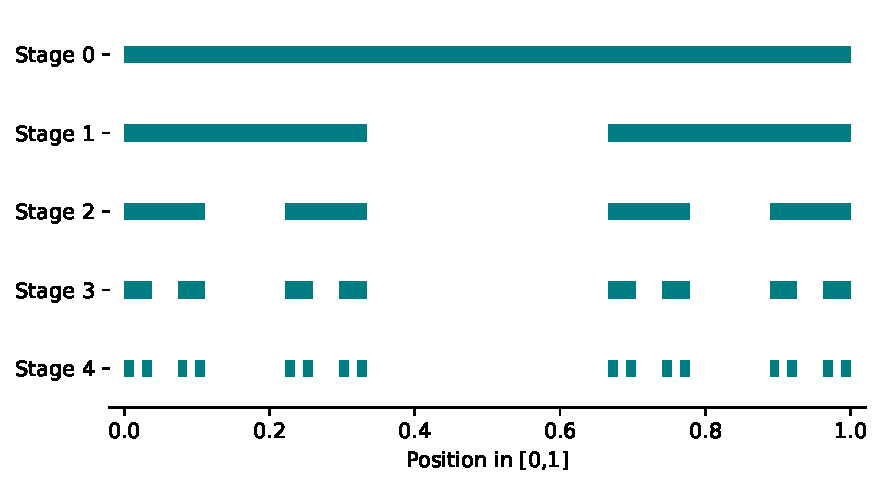
\includegraphics[width=.96\linewidth]{figures/cantor_stages.pdf}\end{center}
At stage $n$, the retained set has $2^n$ intervals, each of length $3^{-n}$. The infinite intersection is not an empty set: it includes zero, one, and every point whose ternary expansion can be chosen using only digits zero and two. The total retained length tends to zero while the final set remains uncountable.
\end{note}


\topic{Further exercise methods from the supplied notes}
\begin{note}{A convergent sequence together with its limit is closed (Exercise 6.5)}
Let $C=\{a\}\cup\{x_n:n\in\N\}$ with $x_n\to a$. For $p\notin C$, let $r=d(p,a)/3>0$. A tail lies in $B_r(a)$, so is at distance at least $2r$ from $p$. The finitely many earlier terms have a positive minimum distance from $p$. Choose a radius below both $r$ and this finite minimum; its ball about $p$ avoids $C$. Thus $E\setminus C$ is open and $C$ is closed. It is also sequentially compact: either one value occurs infinitely often, or a subsequence of the chosen sequence runs to arbitrarily late indices and hence tends to $a$.
\end{note}
\begin{note}{Cauchy tails and separated consecutive subsequence terms}
For $X_n=\{x_k:k\ge n\}$, Cauchyness is equivalent to $\diam X_n\to0$ (Exercise 6.8): each direction follows by translating ``all pairwise tail distances are small'' into the definition of diameter.

For Exercise 5.7, Cauchyness is equivalent to $\forall\varepsilon>0\ \exists N\ \forall n\ge N:d(x_N,x_n)<\varepsilon$. The reverse implication uses the triangle inequality through $x_N$ and starts with $\varepsilon/2$.

If a sequence is not Cauchy, fix $\eta>0$ witnessing this. Given a selected term $x_{n_k}$ and any later cutoff, there are two terms beyond that cutoff at distance at least $\eta$. At least one has distance at least $\eta/2$ from $x_{n_k}$; otherwise their mutual distance would be below $\eta$. Select it as $x_{n_{k+1}}$. This gives a subsequence with consecutive distances bounded below by $\eta/2$. Conversely, such a subsequence prevents Cauchyness.
\end{note}
\begin{note}{Pseudo-metrics and quotient spaces (Exercise 6.9)}
A pseudo-metric satisfies the metric axioms except that distinct points may have zero distance. Define $x\sim y$ iff $\rho(x,y)=0$. Reflexivity and symmetry are immediate; transitivity follows from $\rho(x,z)\le\rho(x,y)+\rho(y,z)=0$.

Define $d([x],[y])=\rho(x,y)$. To check well-definedness, if $x\sim x'$ and $y\sim y'$, then
\[\rho(x,y)\le\rho(x,x')+\rho(x',y')+\rho(y',y)=\rho(x',y'),\]
and the reversed inequality gives equality. Definiteness now holds for equivalence classes; other axioms descend from $\rho$.

For Riemann-integrable functions with $\rho(f,g)=\int_a^b|f-g|$, functions differing at one point can have distance zero. The quotient identifies all pairs with zero integral discrepancy, and the displayed integral defines a true metric on these classes.
\end{note}
\begin{exam}{Additional practice based on Exercise 6.9}
On $\R^2$ define $\rho((x,y),(u,v))=|x-u|$. Describe the equivalence classes and the quotient metric space.
\end{exam}
\begin{answer}
The function is a pseudo-metric, since it is the ordinary distance between first coordinates. It can vanish for distinct points such as $(0,0)$ and $(0,1)$. Two points are equivalent iff their first coordinates agree, so each class is a vertical line. Assign the class of $(x,y)$ to the real number $x$. This is a bijection from the quotient to $\R$, and the quotient distance between two classes is $|x-u|$. Thus the quotient is isometric to the usual real line.
\end{answer}
\begin{note}{One remaining set-theoretic construction (Exercise 4.12)}
Given $c=(c_n)\in\{0,1\}^{\N}$, put $x=\sum_{n\ge1}c_n10^{-n}$. Then $\lfloor10^nx\rfloor=\sum_{k=1}^nc_k10^{n-k}$ because the remaining tail is at most $1/9<1$. All terms except $c_n$ are even; hence the parity of this floor is $c_n$. Therefore the parity-of-decimal-floors map in Exercise 4.12 is surjective onto binary sequence space. Any surjection $\N\to\R$ composed with it would enumerate binary sequence space, contradicting diagonalisation. Here the floor uses integers, including negative integers, as usual.
\end{note}


\topic{Detailed proof: Compact domain makes continuity uniform}
\begin{exam}{Additional practice based on Section 2}
Let $K$ be a sequentially compact metric space and $f:K\to F$ continuous into a metric space. Prove $f$ uniformly continuous.
\end{exam}
\begin{method}{Negate the global claim to obtain two close-input sequences}
Failure of uniform continuity gives one output tolerance that cannot be achieved by any single input tolerance. Choosing input tolerance $1/n$ produces pairs of inputs which are increasingly close but whose outputs remain a fixed distance apart.
\end{method}
\begin{answer}
Suppose $f$ is not uniformly continuous. Then there is $\varepsilon_0>0$ such that, for every $\delta>0$, some $x,y\in K$ satisfy $d_K(x,y)<\delta$ but $d_F(f(x),f(y))\ge\varepsilon_0$. For each $n$ choose such $x_n,y_n$ with
\[d_K(x_n,y_n)<1/n,\qquad d_F(f(x_n),f(y_n))\ge\varepsilon_0.\]
Sequential compactness gives a subsequence $x_{n_j}\to p\in K$. Then
\[d_K(y_{n_j},p)\le d_K(y_{n_j},x_{n_j})+d_K(x_{n_j},p)\to0,\]
so $y_{n_j}\to p$ too. Continuity at $p$ implies $f(x_{n_j})\to f(p)$ and $f(y_{n_j})\to f(p)$. Consequently
\[d_F(f(x_{n_j}),f(y_{n_j}))\le d_F(f(x_{n_j}),f(p))+d_F(f(p),f(y_{n_j}))\to0.\]
But these distances are all at least $\varepsilon_0>0$, a contradiction. Thus $f$ is uniformly continuous.
\end{answer}
\begin{tip}
Compactness is applied only to the first sequence. The closeness of each input pair then forces the corresponding second subsequence to have the same limit. Independently extracting two subsequences could lose the required pairing.
\end{tip}


\topic{Proof clinic: Completeness and compactness: keep the logical arrows separate}
\begin{note}{A complete space need not keep every sequence under control}
Completeness only promises limits for Cauchy sequences. In $\R$, the sequence $n$ has no convergent subsequence, but this does not contradict completeness because it is not Cauchy. Sequential compactness demands a convergent subsequence from \emph{any} sequence, so it is stronger.

In $\R^n$, boundedness is strong enough, via Bolzano--Weierstrass, to obtain a convergent subsequence in the ambient space. Closedness then retains the limit inside the subset. In general metric spaces, boundedness alone does not give that subsequence; total boundedness is what provides successively finer finite covers.

Thus two routes to sequential compactness are available: in finite-dimensional norm metrics, closed and bounded; in general metric spaces, complete and totally bounded. Do not silently use the finite-dimensional route outside its hypotheses.
\end{note}
\begin{exam}{Additional practice: classification table}
Classify $\R$, $(0,1)$, $[0,1]$ and an infinite discrete space for completeness, boundedness and sequential compactness.
\end{exam}
\begin{answer}
\begin{tabular}{p{.32\linewidth}ccc}
\textbf{Usual metric unless stated} & \textbf{Complete} & \textbf{Bounded} & \textbf{Seq. compact}\\[4pt]
$\R$ & Yes & No & No\\[3pt]
$(0,1)$ & No & Yes & No\\[3pt]
$[0,1]$ & Yes & Yes & Yes\\[3pt]
Infinite discrete space & Yes & Yes & No
\end{tabular}

For $\R$, use its completeness theorem and the sequence $n$ to disprove compactness. For $(0,1)$, $1/n$ (starting at $n=2$) is Cauchy but its only ambient limit is missing. For $[0,1]$, use closedness and completeness, then Heine--Borel. For the discrete example, Cauchy sequences are eventually constant but a sequence of distinct points has no convergent subsequence.
\end{answer}


\topic{Proof clinic: Recognising when an infimum becomes an attained minimum}
\begin{exam}{Additional practice: when a distance infimum is attained}
In the metric space $E=(0,\infty)$ with usual metric, let $A=(0,1]$ and $p=2$. Find the nearest point. Then in $E=\R$, give a nonclosed set with a finite unattained point-distance infimum.
\end{exam}
\begin{answer}
For the first case, $d(2,a)=2-a\ge1$ for $0<a\le1$, with equality at $a=1$. Thus $\dist(2,A)=1$ and it is attained. This shows compactness is sufficient for attainment, not necessary in every particular example.

For the requested unattained infimum in $\R$, let $B=(0,1)$ and $p=2$. Then $d(2,b)=2-b>1$ for every $b\in B$. Taking $b_n=1-1/n$ for $n\ge2$ gives distances $1+1/n\to1$. Hence $\dist(2,B)=1$ and no point attains it. The missing endpoint prevents attainment.
\end{answer}
\begin{note}{A stronger warning in a general metric space}
Even closedness alone need not guarantee a nearest point. On $E=\{p,a_1,a_2,\ldots\}$ define $d(p,a_n)=1+1/n$, $d(a_n,a_m)=2$ for distinct $n,m$, and zero on the diagonal. This is a metric: the only potentially smaller two-leg route between distinct $a_n,a_m$ through $p$ has length $2+1/n+1/m>2$; routes from $p$ via another $a_m$ are longer than its direct distances. The subset $A=\{a_n:n\ge1\}$ is closed because $B_1(p)$ avoids it. Yet $\dist(p,A)=1$ is not attained. The set is not sequentially compact, since its points are uniformly separated. This is why the compact attainment theorem carries more information than closedness alone.
\end{note}


\topic{Proof clinic: Two different diagonal arguments}
\begin{note}{Do not confuse construction with extraction}
Cantor's uncountability diagonal changes the $n$th coordinate of the $n$th listed object to produce a new object absent from a proposed list. The purpose is to show no enumeration can be exhaustive.

The compact-product diagonal extracts the $n$th term of the $n$th \emph{nested subsequence}. It produces a subsequence whose tail inherits convergence in every fixed coordinate. The purpose is to make infinitely many coordinate requirements hold simultaneously.

Both inspect a diagonal array, but their logical jobs differ. In the second argument, the rows must be nested subsequences. Taking a diagonal from unrelated convergent coordinate sequences does not necessarily produce a subsequence of the original product sequence.
\end{note}
\begin{exam}{Additional practice: a compact-product sequence}
In $\{0,1\}^{\N}$ with $D(x,y)=\sum_i2^{-i}|x_i-y_i|$, let $x^{(n)}$ have its first $n$ coordinates equal to $1$ and the rest zero. Find its limit and the exact distance to it.
\end{exam}
\begin{answer}
The candidate limit is $a=(1,1,1,\ldots)$. For each fixed coordinate $i$, $x_i^{(n)}=1$ once $n\ge i$, so coordinatewise convergence holds. Directly,
\[D(x^{(n)},a)=\sum_{i>n}2^{-i}=2^{-n}\to0.\]
Thus the sequence converges to $a$ in the weighted product metric. In contrast, its unweighted sup distance from $a$ is $1$ for every $n$, because there are always later coordinates still equal to zero. The metric determines which kind of convergence is being discussed.
\end{answer}


\topic{Worked lecture exercises}
\exercise{6.1}{Finite sets, unions and intersections}
\begin{exam}{Lecture exercise}
Show finite sets are sequentially compact and the union and intersection of two sequentially compact sets are sequentially compact.
\end{exam}
\begin{answer}
If $A$ is finite and $(x_n)$ a sequence in $A$, some point $a\in A$ occurs infinitely often by the infinite pigeonhole principle. Select its indices in increasing order to get a constant subsequence, which converges to $a\in A$. Thus finite sets are sequentially compact. The empty case is vacuous.

Let $A,B$ sequentially compact and $(x_n)$ a sequence in $A\cup B$. Either infinitely many terms lie in $A$, or only finitely many do, in which case infinitely many lie in $B$. Select a subsequence lying entirely in one constituent. Its sequential compactness gives a further subsequence converging to a point of that constituent, hence of $A\cup B$. Therefore the union is sequentially compact.

For the intersection, start with a sequence in $A\cap B$. Since it lies in $A$, choose a subsequence converging to $a\in A$. Sequentially compact $B$ is closed in the ambient metric space. All selected terms lie in $B$, so their limit $a$ lies in $B$ too. Hence $a\in A\cap B$, proving sequential compactness of the intersection.
\end{answer}
\begin{tip}
The intersection argument uses closedness of one compact set. It is unnecessary to extract a second subsequence, although that alternative also works with uniqueness of limits.
\end{tip}
\exercise{6.2}{A closest point in a compact set}
\begin{exam}{Lecture exercise}
For nonempty sequentially compact $K$ and $p\in E$, prove there exists $c\in K$ with $d(c,p)=\dist(p,K)$.
\end{exam}
\begin{answer}
Let $r=\dist(p,K)=\inf_{x\in K}d(p,x)$. It is a finite nonnegative real because $K$ is nonempty and distances are finite. By infimum approximation choose $x_n\in K$ such that
\[r\le d(p,x_n)<r+1/n.\]
Then $d(p,x_n)\to r$. Sequential compactness gives a subsequence $x_{n_j}\to c\in K$. Reverse triangle inequality shows $|d(p,x_{n_j})-d(p,c)|\le d(x_{n_j},c)\to0$, so this subsequence of distance values tends to $d(p,c)$. It also tends to $r$, since the whole distance sequence does. Uniqueness of real limits gives $d(p,c)=r$, as required.
\end{answer}
\begin{method}{Approximate, extract, pass to the limit}
This three-step pattern proves many attainment theorems. The infimum first gives approximate minimisers; compactness gives a convergent subsequence; continuity turns its limiting value into an actual minimiser.
\end{method}
\exercise{6.3}{Continuous functions attain extrema}
\begin{exam}{Lecture exercise}
For continuous $f:E\to\R$ and nonempty sequentially compact $K\subseteq E$, prove $f$ attains its maximum and minimum on $K$.
\end{exam}
\begin{answer}
First $f[K]$ is sequentially compact by the continuous-image theorem, and hence bounded. Therefore $s=\sup f[K]$ and $l=\inf f[K]$ are finite reals.

By supremum approximation choose $x_n\in K$ with $s-1/n<f(x_n)\le s$. Thus $f(x_n)\to s$. Sequential compactness supplies $x_{n_j}\to q\in K$. Continuity gives $f(x_{n_j})\to f(q)$. Since the same subsequence of values tends to $s$, uniqueness yields $f(q)=s$. Thus the supremum is attained.

Apply the same argument to $-f$, which is continuous. It has a maximiser $p\in K$. Then $-f(x)\le-f(p)$ for all $x\in K$, which means $f(p)\le f(x)$. Therefore
\[f(p)\le f(x)\le f(q)\quad\text{for all }x\in K.\]
\end{answer}
\begin{tip}
Nonemptiness is needed for attaining points. The empty set is sequentially compact but supplies neither a maximiser nor a minimiser.
\end{tip}
\exercise{6.4}{Bounded means fitting inside a box}
\begin{exam}{Lecture exercise}
For $A\subseteq\R^N$, prove boundedness in $d_\infty$ iff $A\subseteq[-L,L]^N$ for some finite $L\ge0$.
\end{exam}
\begin{answer}
If $A=\varnothing$, choose $L=0$. Assume $A\ne\varnothing$ and $\diam_\infty A=D<\infty$. Choose $a\in A$. For each $x\in A$,
\[\norm{x}_\infty\le\norm{x-a}_\infty+\norm{a}_\infty\le D+\norm{a}_\infty.\]
Set $L=D+\norm{a}_\infty$. Since every coordinate has modulus at most $\norm{x}_\infty\le L$, $x\in[-L,L]^N$, proving containment.

Conversely, if every coordinate of every point has modulus at most $L$, then for $x,y\in A$ each coordinate difference satisfies $|x_i-y_i|\le2L$. Taking the maximum gives $d_\infty(x,y)\le2L$, so $\diam_\infty A\le2L<\infty$. Thus $A$ is bounded.
\end{answer}
\exercise{6.5}{A convergent sequence with its limit is closed}
\begin{exam}{Lecture exercise}
If $x_n\to a$ in $E$, prove $C=\{a\}\cup\{x_n:n\in\N\}$ is closed.
\end{exam}
\begin{method}{Separate the tail from the finite beginning}
For a point $p\notin C$, the limit $a$ is at positive distance from $p$. Late terms cluster near $a$, leaving room around $p$. Only finitely many early terms remain to avoid.
\end{method}
\begin{answer}
Fix $p\in E\setminus C$. Since $p\ne a$, let $r=d(p,a)/3>0$. Choose $N$ such that $d(x_n,a)<r$ for all $n\ge N$. Reverse triangle inequality gives
\[d(p,x_n)\ge d(p,a)-d(a,x_n)>3r-r=2r\quad(n\ge N).\]
Every early term is distinct from $p$, so all distances $d(p,x_i)$ for $i<N$ are positive. Define
\[s=\min\bigl(\{r\}\cup\{d(p,x_i)/2:1\le i<N\}\bigr)>0.\]
A point within distance $s$ of $p$ cannot equal $a$, since $d(p,a)=3r>s$; cannot equal a tail term, since those have distance above $2r\ge2s$; and cannot equal an early term, since its distance is at least $2s$. Hence $B_s(p)\cap C=\varnothing$. Thus every point outside $C$ has a ball outside $C$, so the complement is open and $C$ is closed.
\end{answer}
\exercise{6.6}{Composition of continuous maps}
\begin{exam}{Lecture exercise}
For continuous $f:E\to F$ and $g:F\to G$, prove $g\circ f$ continuous.
\end{exam}
\begin{answer}
Fix $p\in E$ and $\varepsilon>0$. By continuity of $g$ at $f(p)$ there is $\eta>0$ such that $d_F(y,f(p))<\eta$ implies $d_G(g(y),g(f(p)))<\varepsilon$. By continuity of $f$ at $p$ there is $\delta>0$ such that $d_E(x,p)<\delta$ implies $d_F(f(x),f(p))<\eta$. Combining the two implications gives
\[d_E(x,p)<\delta\Rightarrow d_G(g(f(x)),g(f(p)))<\varepsilon.\]
Thus the composition is continuous at arbitrary $p$.

Equivalently, for open $U\subseteq G$, $(g\circ f)^{-1}[U]=f^{-1}[g^{-1}[U]]$ is open because each inverse-image step preserves openness.
\end{answer}
\begin{tip}
Choose tolerances in reverse order: first what $g$ needs in its input, then what $f$ needs to achieve that tolerance. This is why $\eta$ is selected before $\delta$.
\end{tip}
\exercise{6.7}{The identity theorem}
\begin{exam}{Lecture exercise}
For continuous $f,g:E\to F$, prove their agreement set is closed. Deduce that agreement on a dense subset implies agreement everywhere.
\end{exam}
\begin{answer}
Let $H=\{x\in E:f(x)=g(x)\}$. Take a sequence $x_n\in H$ converging in $E$ to $x$. Then continuity gives $f(x_n)\to f(x)$ and $g(x_n)\to g(x)$. Since $f(x_n)=g(x_n)$ for every $n$, these are the same sequence; uniqueness of limits in $F$ gives $f(x)=g(x)$. Therefore $x\in H$, proving $H$ closed.

Now suppose $D$ is dense in $E$ and $f=g$ on $D$. Then $D\subseteq H$, so closure monotonicity gives $E=\cl D\subseteq\cl H=H$. Since $H\subseteq E$ already, $H=E$. Thus $f=g$ on all of $E$.
\end{answer}
\begin{note}{Where you use this result}
It supplies uniqueness of continuous extensions from dense sets, including the extension theorem and uniqueness of completion maps. The values on a dense set determine a continuous function everywhere.
\end{note}
\exercise{6.8}{Diameters of tails}
\begin{exam}{Lecture exercise}
For $X_n=\{x_k:k\ge n\}$, prove $(x_n)$ is Cauchy iff $\diam X_n\to0$.
\end{exam}
\begin{answer}
Assume Cauchy and fix $\varepsilon>0$. Choose $N$ such that $d(x_j,x_k)<\varepsilon/2$ for $j,k\ge N$. Every pair in $X_N$ satisfies this, so taking a supremum gives $\diam X_N\le\varepsilon/2$. Since $X_n\subseteq X_N$ for $n\ge N$, diameter monotonicity gives $\diam X_n\le\varepsilon/2<\varepsilon$ for $n\ge N$. Thus the tail diameters tend to zero.

Conversely, suppose $\diam X_n\to0$. Given $\varepsilon>0$, choose $N$ with $\diam X_N<\varepsilon$. For $j,k\ge N$, both $x_j,x_k\in X_N$, so $d(x_j,x_k)\le\diam X_N<\varepsilon$. This is exactly Cauchyness.
\end{answer}
\begin{tip}
An infinite supremum of numbers strictly below $\varepsilon$ may equal $\varepsilon$. Starting with $\varepsilon/2$ makes the first implication's strict final bound safe.
\end{tip}
\exercise{6.9}{Turning a pseudo-metric into a metric}
\begin{exam}{Lecture exercise}
Let $\rho$ satisfy all metric axioms except that zero need not force equality. Prove $x\sim y$ iff $\rho(x,y)=0$ is an equivalence relation, and $d([x],[y])=\rho(x,y)$ is a well-defined metric. Interpret this for integral discrepancy on Riemann-integrable functions.
\end{exam}
\begin{method}{Well-definedness must precede metric axioms}
A point of the quotient is an equivalence class, which has many possible representatives. Before declaring a distance, prove that changing either representative does not change the formula's value.
\end{method}
\begin{answer}
Reflexivity holds because $\rho(x,x)=0$. Symmetry follows from $\rho(x,y)=\rho(y,x)$. If $x\sim y$ and $y\sim z$, triangle inequality gives $0\le\rho(x,z)\le\rho(x,y)+\rho(y,z)=0$, so $x\sim z$. Thus $\sim$ is an equivalence relation.

If $x\sim x'$ and $y\sim y'$, then
\[\rho(x,y)\le\rho(x,x')+\rho(x',y')+\rho(y',y)=\rho(x',y').\]
Interchanging primed and unprimed points gives the reverse inequality, hence equality. The formula for $d$ is therefore independent of representatives.

Its values are finite and nonnegative. It is symmetric because $\rho$ is. Also $d([x],[y])=0$ iff $x\sim y$ iff $[x]=[y]$, giving definiteness on classes. For any third class $[z]$,
\[d([x],[z])=\rho(x,z)\le\rho(x,y)+\rho(y,z)=d([x],[y])+d([y],[z]).\]
Thus it is a metric.

For Riemann-integrable functions on a nondegenerate $[a,b]$, $\rho(f,g)=\int_a^b|f-g|$ is a pseudo-metric. For example $f\equiv0$ and $g$ equal to $1$ at one point and $0$ elsewhere are distinct with zero discrepancy. The quotient identifies all functions whose absolute difference has integral zero; the distance between their classes is that integral. It is now a true metric because zero distance means equality of classes, not equality at every input.
\end{answer}
\begin{tip}
Do not confuse a quotient class with a chosen function. The quotient construction deliberately treats some different pointwise functions as the same point, repairing the failed definiteness axiom.
\end{tip}

\topic{Past-paper navigation and source register}
\begin{note}{2022 paper: where to revise each question}
\begin{tabular}{p{.18\linewidth}p{.73\linewidth}}
Q1 & Balls, isometries and Lipschitz maps: four equidistant planar points.\\[3pt]
Q2(a)--(b) & Open sets and interior: definition and unions of open/closed balls.\\[3pt]
Q2(c)--(d) & Metric subspaces and relative topology: restricted metric and relative-open-set proof.\\[3pt]
Q3(a)--(b) & Completeness and closed subspaces: definitions, homeomorphism and uniform-continuity transfer.\\[3pt]
Q3(c) & Banach theorem and contraction iterates: complete model proof.\\[3pt]
Q4(a)--(b) & Sequential compactness and continuous images.\\[3pt]
Q4(c) & Continuous images, extrema and inverse continuity: compact self-isometry.
\end{tabular}
\end{note}
\begin{note}{2023 paper: where to revise each question}
\begin{tabular}{p{.18\linewidth}p{.73\linewidth}}
Q1 & Discrete metric and equilateral three-point embedding.\\[3pt]
Q2(a) & Norms, norm-induced metrics and the matrix norm model answer.\\[3pt]
Q2(b) & Closed sets, closure and boundary: closure of finite unions and intersection counterexample.\\[3pt]
Q2(c) & Continuity: definition, open-preimage theorem, constant-image counterexample.\\[3pt]
Q3(a) & Density: dense intersect open dense, and disjoint dense counterexample.\\[3pt]
Q3(b) & Function metrics and completeness of sup spaces.\\[3pt]
Q4(a) & Continuous images: bounded/closed counterexamples and Heine--Borel.\\[3pt]
Q4(b) & Finite and countable products: weighted sup metric, full model proof.
\end{tabular}
\end{note}
\begin{note}{2024 paper: where to revise each question}
\begin{tabular}{p{.18\linewidth}p{.73\linewidth}}
Q1 & Discrete metric, exact ball radii, eventual constancy.\\[3pt]
Q2(a)--(c) & Open sets, complements, subspaces, relative clopen example.\\[3pt]
Q2(d)(i)--(iv) & Open unions, infinite-intersection counterexample, density.\\[3pt]
Q2(d)(v) & Countable dense dyadic polygonal family in $C([0,1])$.\\[3pt]
Q3(a)--(c) & Equivalent metrics: Cauchy equivalence, truncation and arctangent.\\[3pt]
Q3(d) & Completeness of $\ell^\infty(S;[0,1])$.\\[3pt]
Q4(a) & Sequential compactness, image theorem, bounded sets in balls.\\[3pt]
Q4(b) & Product compactness and Heine--Borel: compact unit ball argument.
\end{tabular}
\end{note}
\begin{note}{2025 paper: where to revise each question}
\begin{tabular}{p{.18\linewidth}p{.73\linewidth}}
Q1 & Triangle estimates: full four-point and reverse-triangle arguments.\\[3pt]
Q2 & Countability: definition and binary diagonal proof.\\[3pt]
Q3(a)--(d) & Open/closed/continuous definitions, openness of balls, disjoint balls and proper open set.\\[3pt]
Q3(e)--(f) & Closed complement proof and inverse-open-set characterisation.\\[3pt]
Q4(a) & Completeness iff closedness in a complete ambient space.\\[3pt]
Q4(b) & Complete continuous-function space: bounded image plus uniform limits.\\[3pt]
Q5 & Total boundedness: all three parts worked immediately after the topic.
\end{tabular}
\end{note}
\begin{note}{Source register and coverage}
The following twelve supplied PDFs and the recovered original Section 1 PDF were used. Page references here are physical PDF pages, not the miniature slide numbers printed within pages.
\begin{enumerate}
\item \texttt{MS+T.Section0}: 8 PDF pages. Metric axioms and examples; Exercises 0.1--0.6.
\item \texttt{MS+T.Section1.singleSB}: 26 pages, recovered from the earlier upload dated 15 October 2026. Sets, functions, equivalence relations, countability and optional order theory; Exercises 1.1--1.19.
\item \texttt{MS+T.Section2}: 27 pages. Real analysis, linear algebra, continuity and integration; Exercises 2.1--2.10.
\item \texttt{MS+T.Section3}: 15 pages. Metrics, balls, Lipschitz maps, boundedness, sequences and function spaces; Exercises 3.1--3.14.
\item \texttt{MS+T.Section4}: 17 pages. Topology, density, continuity, subspaces, metric equivalence and products; Exercises 4.1--4.12.
\item \texttt{MS+T.Section5}: 16 pages. Completeness, extensions, completion, Banach, integral equations, Cantor intersection and Baire; Exercises 5.1--5.9.
\item \texttt{MS+T.Section6}: 11 pages. Sequential compactness, products, Heine--Borel and Cantor set; Exercises 6.1--6.9.
\item \texttt{MTS.AppendixOne.ProofOfMinkowski.Inequality}: 3 pages, non-examinable.
\item \texttt{MTS.AppendixTwo.LipschitzExtensionTheorem}: 2 pages, non-examinable.
\item \texttt{MATH316Exam2022.pdf}: 3 pages; all four main questions mapped above.
\item \texttt{MATH316.pdf}: the 2023 paper, 6 pages including information sheet; all four main questions mapped above.
\item \texttt{MATH316MetricSpacesMainSummer2024.pdf}: 6 pages including information sheet; all four main questions mapped above.
\item \texttt{2024-25.FinalisedMATH316.Exam.pdf}: the 2025 paper, 6 pages including information sheet; all five main questions mapped above.
\end{enumerate}
The narrative consolidates repeated definitions and results. The numbered exercise workbooks added to this edition give solutions to all 79 exercises in the Sections 0--6. Non-examinable and optional material retains its status. The guide is a teaching resource, not an official solution manual.
\end{note}
\begin{tip}
Before an exam, reproduce the definition boxes without looking. Practise the open-ball, complement, relative-open-set, dense-intersection, sup-space completeness, uniform-limit, Banach and continuous-image proofs. Then do the four papers under the actual instructions on each paper. Their recurring topics guide practice priorities, but do not establish what a future paper will ask.
\end{tip}

